

\section{Experiments}
\label{sec:exp}
\subsection{Settings}
\label{sec:settings}
 %\subsubsection{Base Models}
{\bf Base Models.} We employ two open-source base models: Llama-3.1-8B-Instruct~\cite{llama3} and Mistral-7B-instruct-v0.2~\cite{jiang2023mistral}. These models, widely adopted due to moderate parameter sizes and impressive performance on long-sequence tasks, both leverage the GQA~\cite{GQA} technique, which reduces the KV cache size to one-quarter of its original.

%\subsubsection{Datasets}
{\bf Datasets.} We conduct evaluations using two popular benchmarks: Ruler~\cite{hsieh2024ruler} and LongBench~\cite{bai2023longbench}. Ruler includes 13 long-sequence tasks, primarily variations of the Needle-in-a-Haystack test, offering a range of difficulty levels for comprehensive model assessment. According to the official evaluation~\cite{hsieh2024ruler}, the maximum effective length for Mistral-7B-instruct-v0.2 and Llama-3.1-8B-Instruct with the full KV Cache is 16K. Therefore, we select the 16K Ruler Benchmark as the primary benchmark for evaluation. Additionally, we also conduct evaluations using LongBench, including 16 datasets covering multiple task domains. Detailed dataset information is provided in Appendix \ref{apdx:ruler_info} and \ref{apdx:longbench_info}. 
%All datasets are assessed using official-recommended metrics, with score up to 100.



%\subsubsection{Baselines}
{\bf Baselines.} We select the \textit{SnapKV}\cite{SnapKV} and \textit{Pyramid}\cite{PyramidInfer, PyramidKV} as the primary baselines, given that they are SOTA methods and foundational bases for our \textit{Ada-SnapKV} and \textit{Ada-Pyramid} methods. All these methods implement GQA compatibility as stated in Section~\ref{sec:imp}, reducing cache size to a quarter of previous naive implementations.
Additionally, \textit{StreamingLLM}~\cite{SLM} is also included as a representative of Sliding Window Eviction Methods for reference.






{\bf Parameters.} Cache eviction methods can be applied whenever KV cache compression is required. Following standard practices in prior studies~\cite{SnapKV, PyramidInfer, PyramidKV}, we perform cache eviction after the prefilling phase of each layer for consistent comparison. In all experiments, the hyperparameter $\alpha$ for adaptive budget allocation is fixed at 0.2. Both \textit{Ada-SnapKV} and \textit{Ada-Pyramid}, as well as \textit{SnapKV} and \textit{Pyramid}, follow the configuration settings outlined in \cite{SnapKV}, including an observation window size of 32 and a max pooling kernel size of 7. 

\begin{figure*}[t!]
	\vspace{-0.1cm}
	\begin{minipage}{\linewidth}
	\centering
	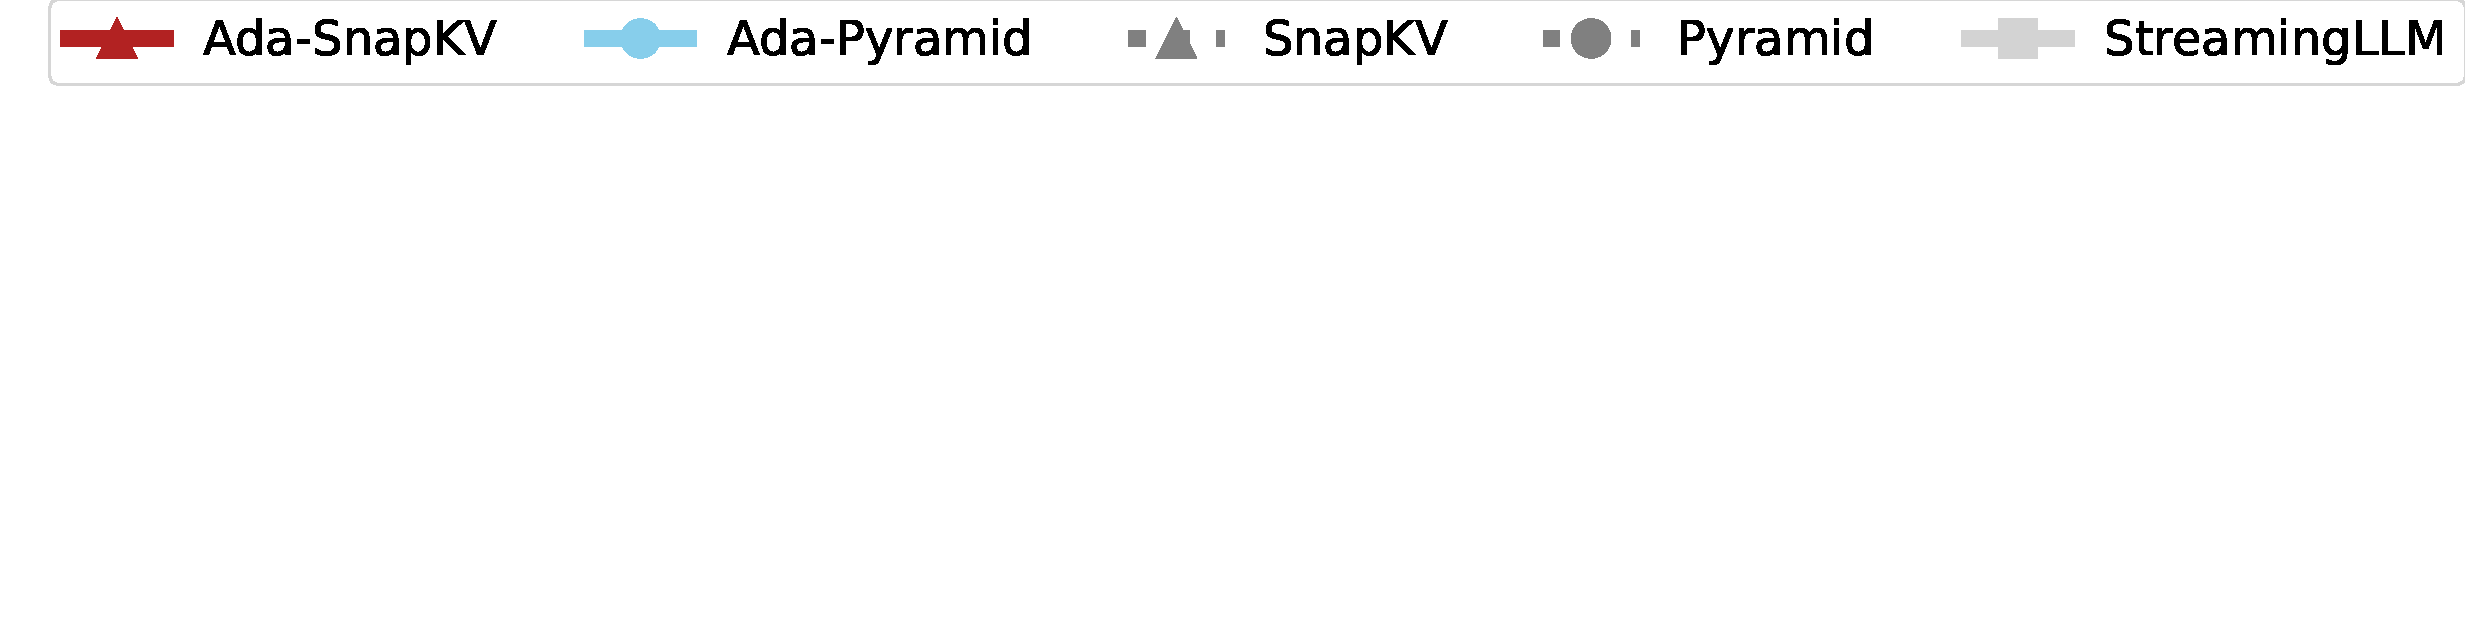
\includegraphics[width=0.85\linewidth]{./Figures/ruler_per_dataset_group_by_wq/legend.pdf}
	\end{minipage}
	\centering
	\begin{subfigure}[b]{0.24\linewidth}
		\centering
		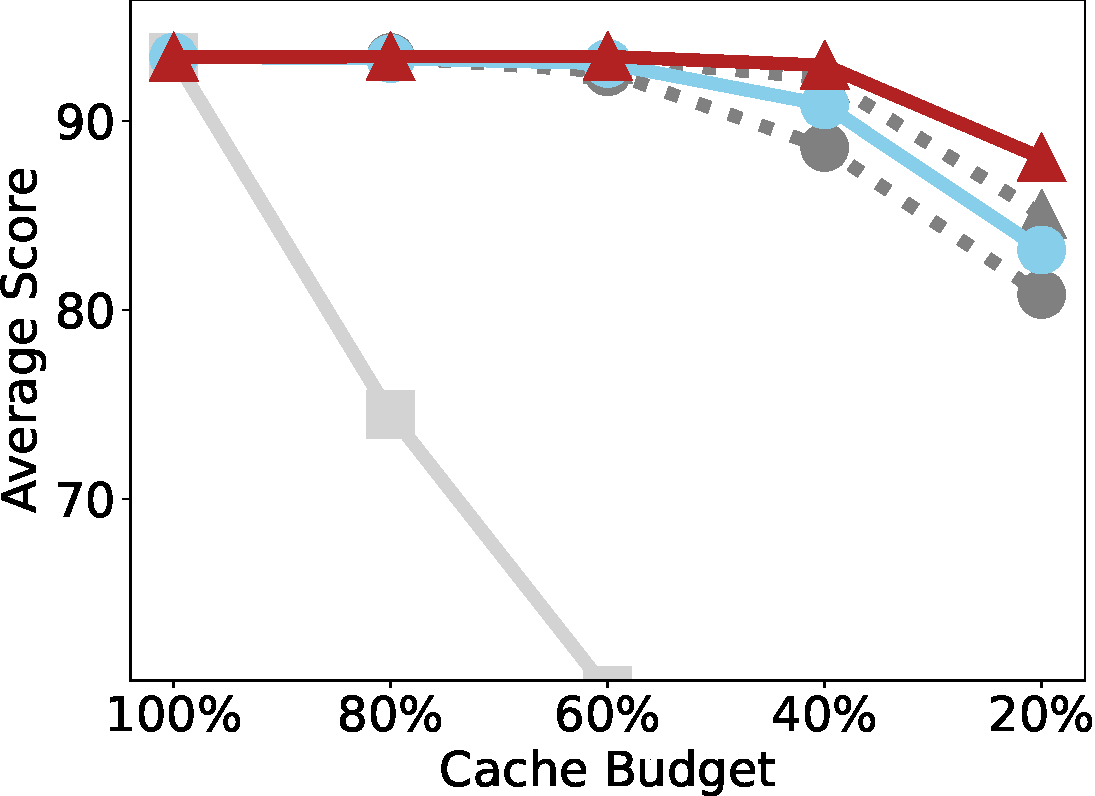
\includegraphics[width=\linewidth]{./Figures/ruler_per_dataset_group_by_wq/average_score_wq_Llama3.1_ruler_score.pdf}
		\vspace{-0.4cm}
		\caption{\centering  Question-aware, \newline Llama-3.1-8B-Instruct}
		\label{fig:aware_llama}
	\end{subfigure}
	\begin{subfigure}[b]{0.24\linewidth}
		\centering
		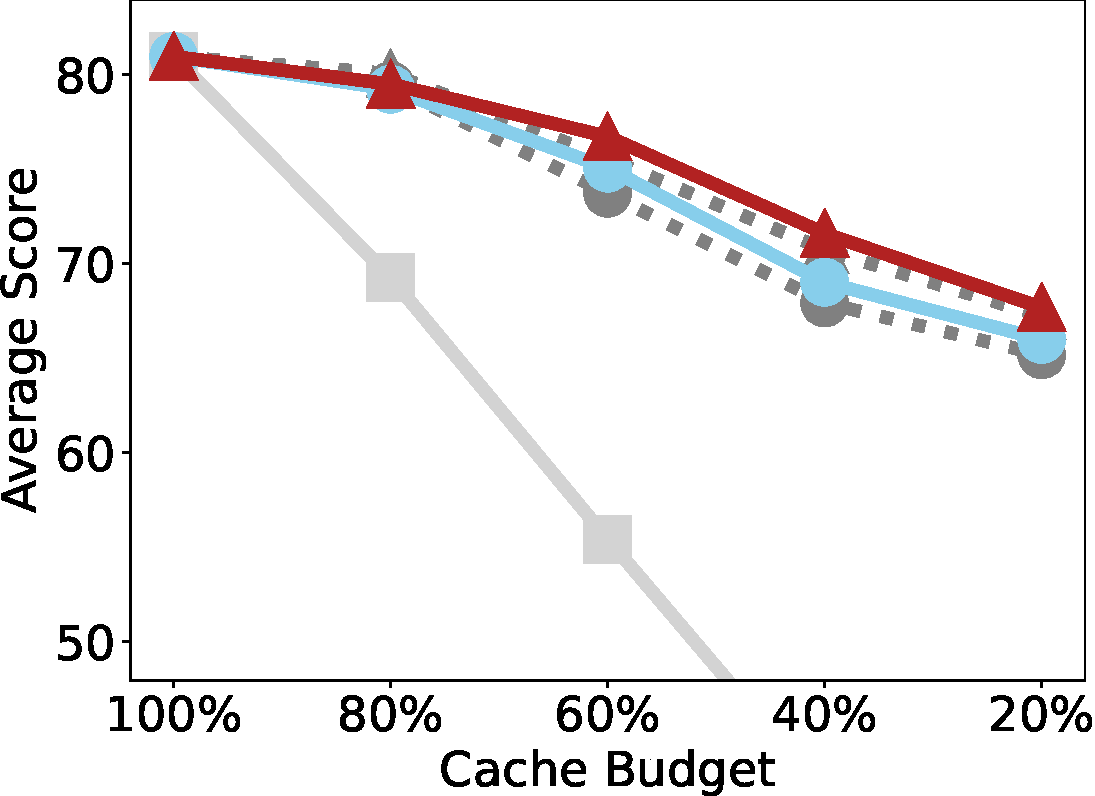
\includegraphics[width=\linewidth]{./Figures/ruler_per_dataset_group_by_wq/average_score_wq_Mistral_ruler_score.pdf}
		\vspace{-0.4cm}
		\caption{\centering  Question-aware, \newline Mistral-7B-Instruct-v0.2}
	\end{subfigure}
	\begin{subfigure}[b]{0.24\linewidth}
		\centering
		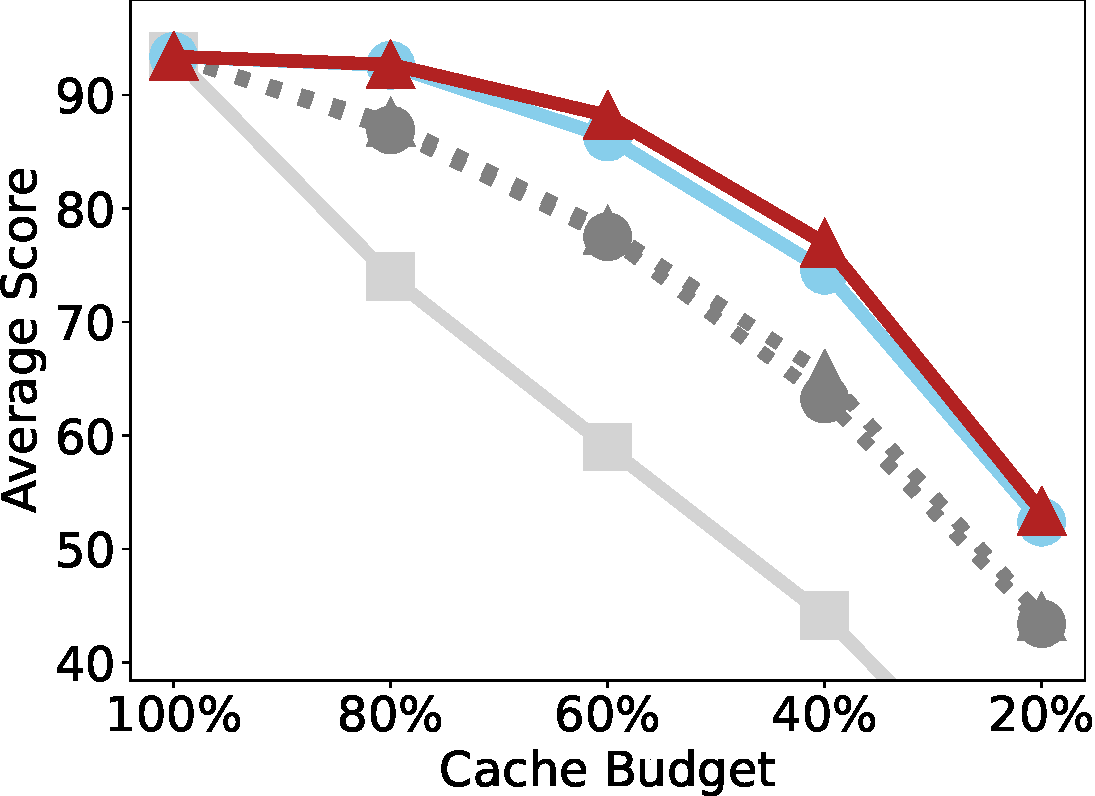
\includegraphics[width=\linewidth]{./Figures/ruler_per_dataset_group_by_wq/average_score_Llama3.1_ruler_score.pdf}
		\vspace{-0.4cm}
		\caption{ \centering  Question-agnostic, \newline Llama-3.1-8B-Instruct}
		\label{fig:agnostic_llama}
	\end{subfigure}
	\begin{subfigure}[b]{0.24\linewidth}
		\centering
		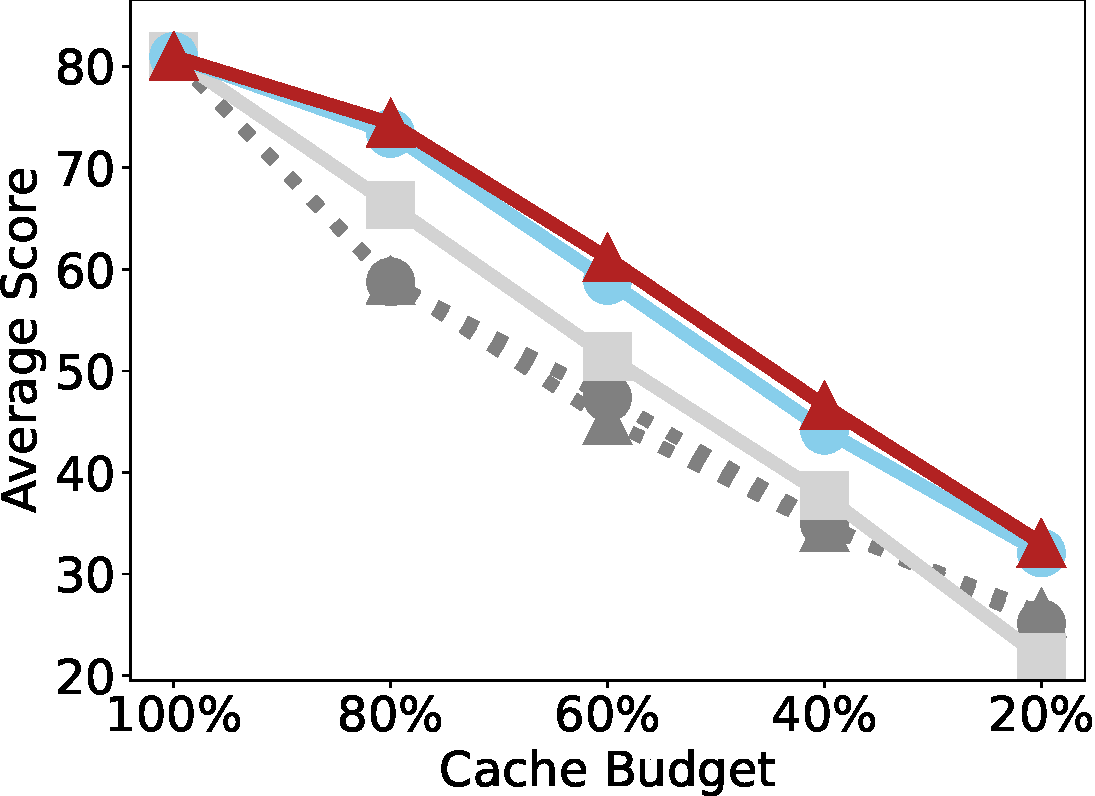
\includegraphics[width=\linewidth]{./Figures/ruler_per_dataset_group_by_wq/average_score_Mistral_ruler_score.pdf}
		\vspace{-0.4cm}
		\caption{ \centering Question-agnostic, \newline Mistral-7B-Instruct-v0.2}
	\end{subfigure}
	\vspace{-0.1cm}
	\caption{Average Score on Ruler Among 13 Datasets.}
	\label{fig:ruler_ave}
	\vspace{-0.2cm}
\end{figure*}
	
\begin{figure*}[t!]
	\vspace{-0.1cm}
	\begin{minipage}{\linewidth}
	\centering
	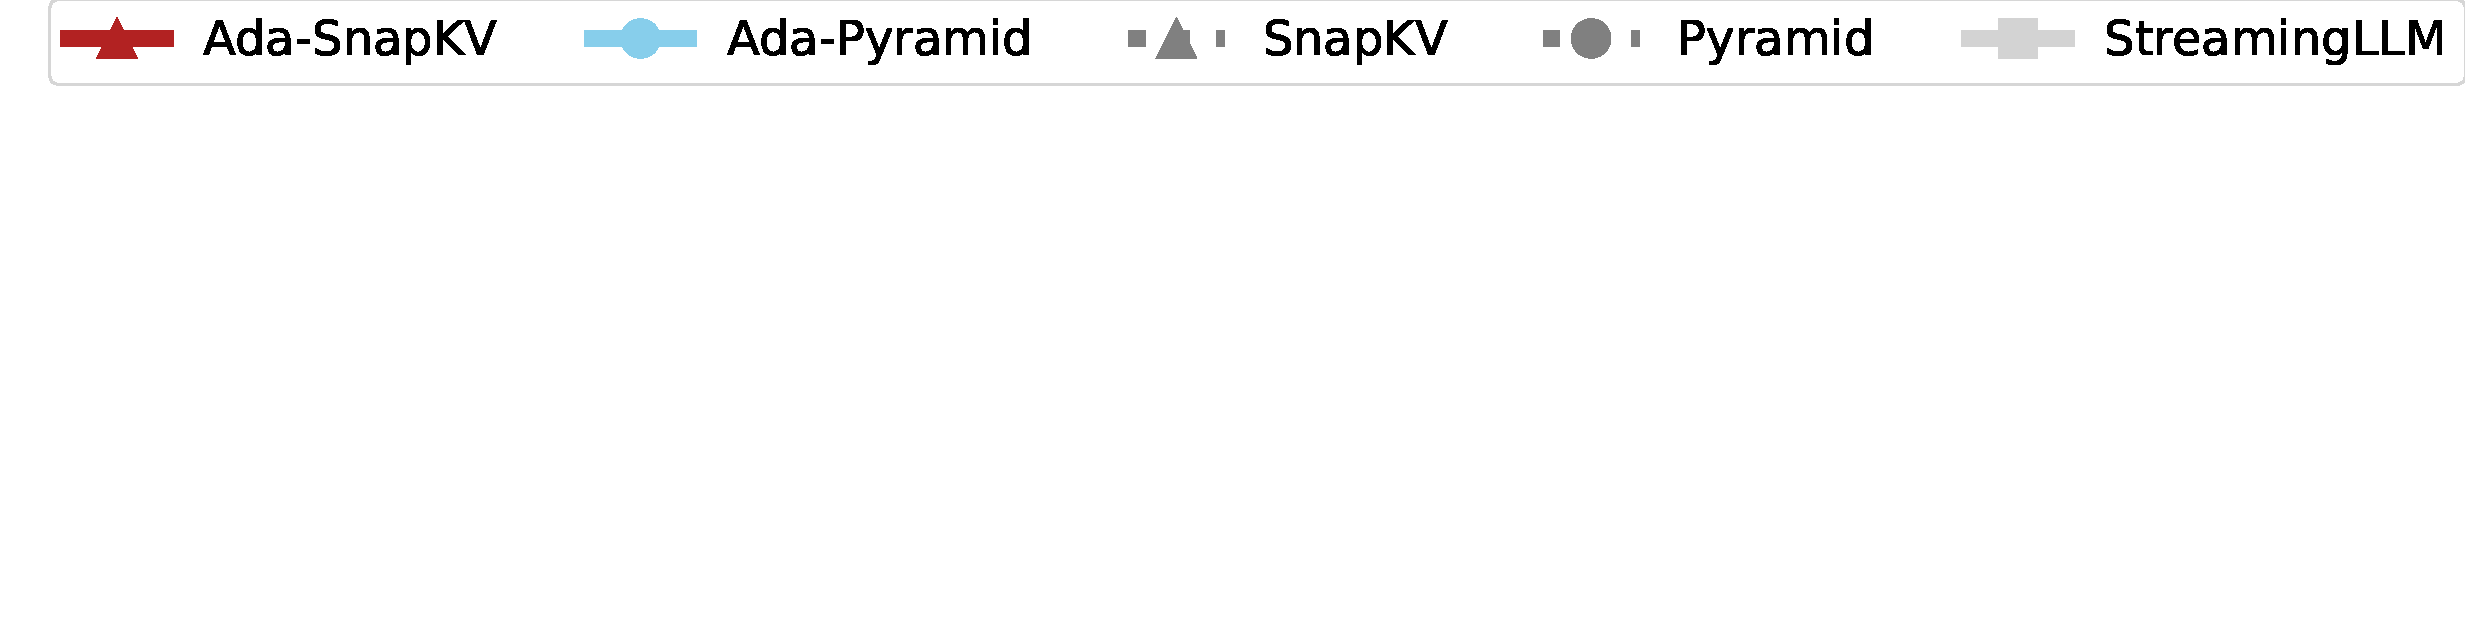
\includegraphics[width=0.85\linewidth]{./Figures/ruler_per_dataset_group_by_wq/legend.pdf}
	\end{minipage}
	\begin{subfigure}[b]{0.16\linewidth}
	\centering
	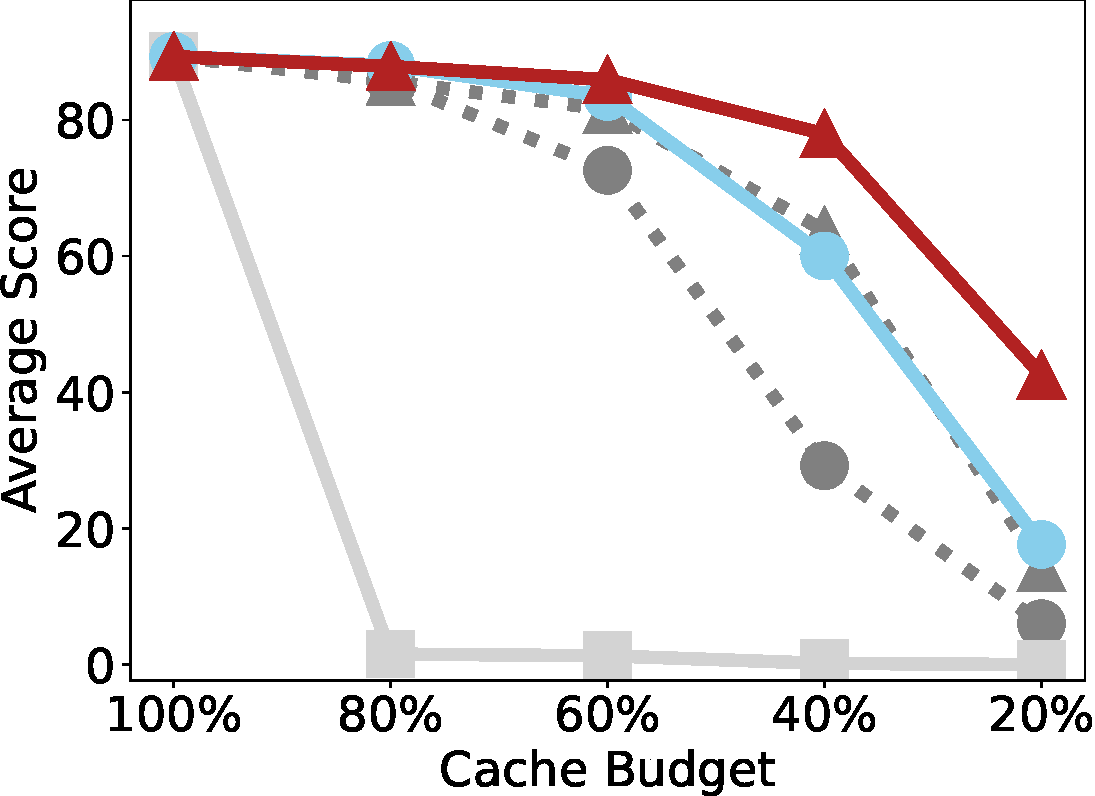
\includegraphics[width=\linewidth]{./Figures/ruler_per_dataset_group_by_wq/cwe_Llama3.1_ruler_score.pdf}
    \vspace{-0.4cm}
	\caption{CWE}
	\end{subfigure}
	\begin{subfigure}[b]{0.16\linewidth}
	\centering
	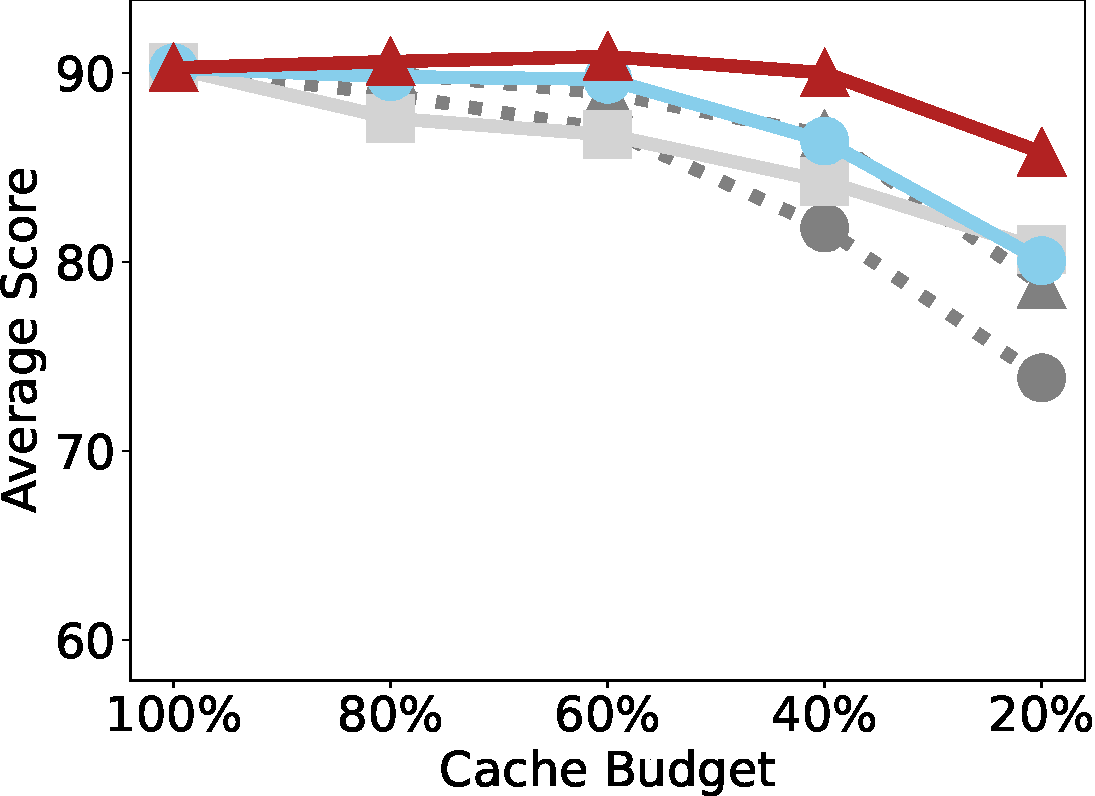
\includegraphics[width=\linewidth]{./Figures/ruler_per_dataset_group_by_wq/fwe_Llama3.1_ruler_score.pdf}
	\vspace{-0.4cm}
	\caption{FWE}
	\end{subfigure}
	\begin{subfigure}[b]{0.16\linewidth}
	\centering
	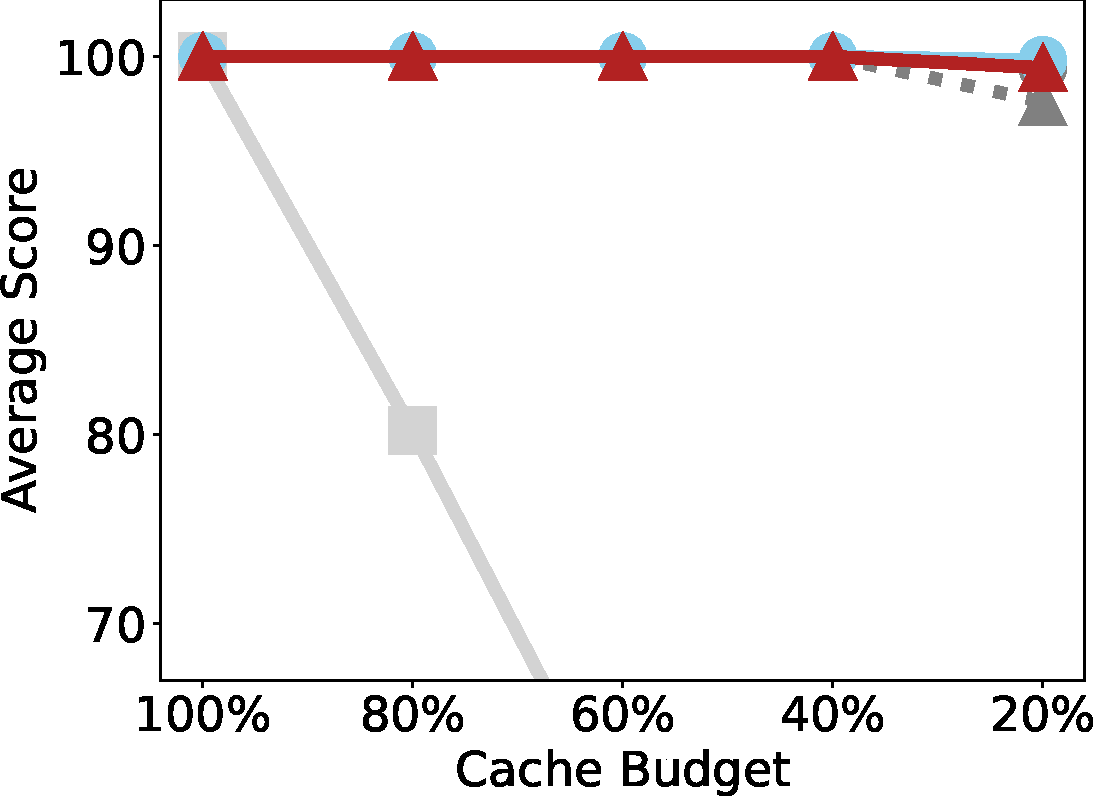
\includegraphics[width=\linewidth]{./Figures/ruler_per_dataset_group_by_wq/niah_single_1_Llama3.1_ruler_score.pdf}
	\vspace{-0.4cm}
	\caption{S-NIAH-1}
	\end{subfigure}
	\begin{subfigure}[b]{0.16\linewidth}
	\centering
	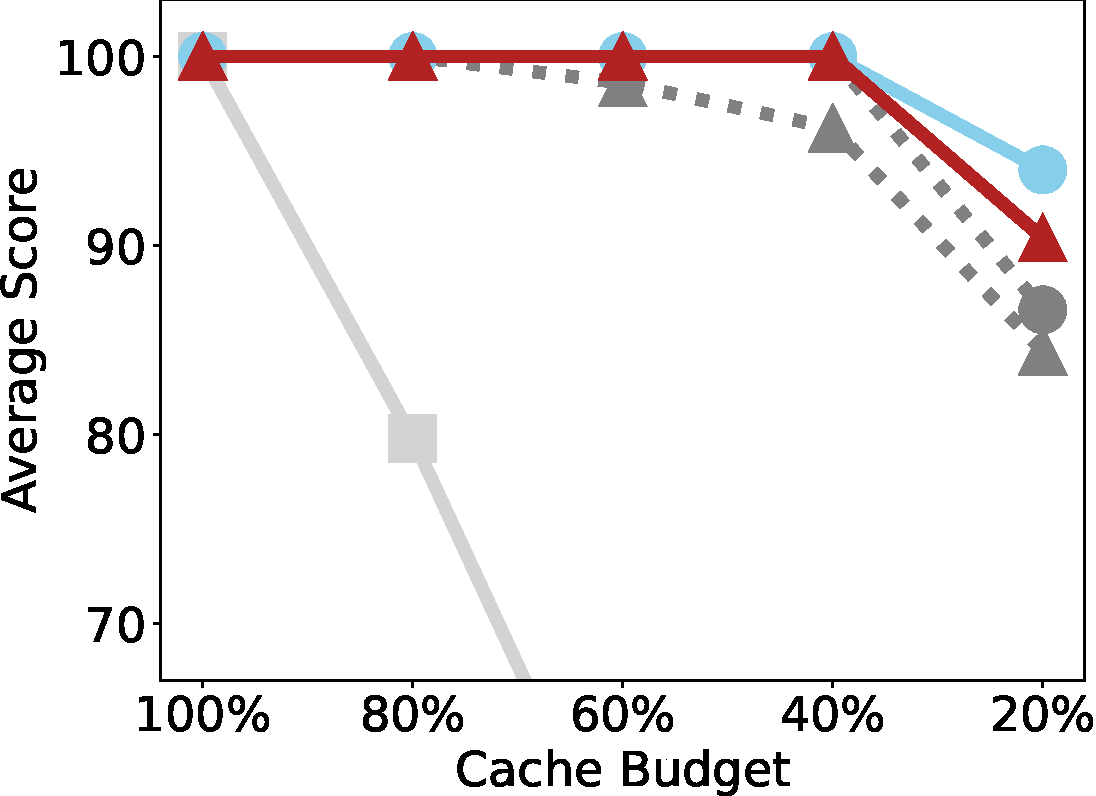
\includegraphics[width=\linewidth]{./Figures/ruler_per_dataset_group_by_wq/niah_single_2_Llama3.1_ruler_score.pdf}
	\vspace{-0.4cm}
	\caption{S-NIAH-2}
	\end{subfigure}
	\begin{subfigure}[b]{0.16\linewidth}
	\centering
	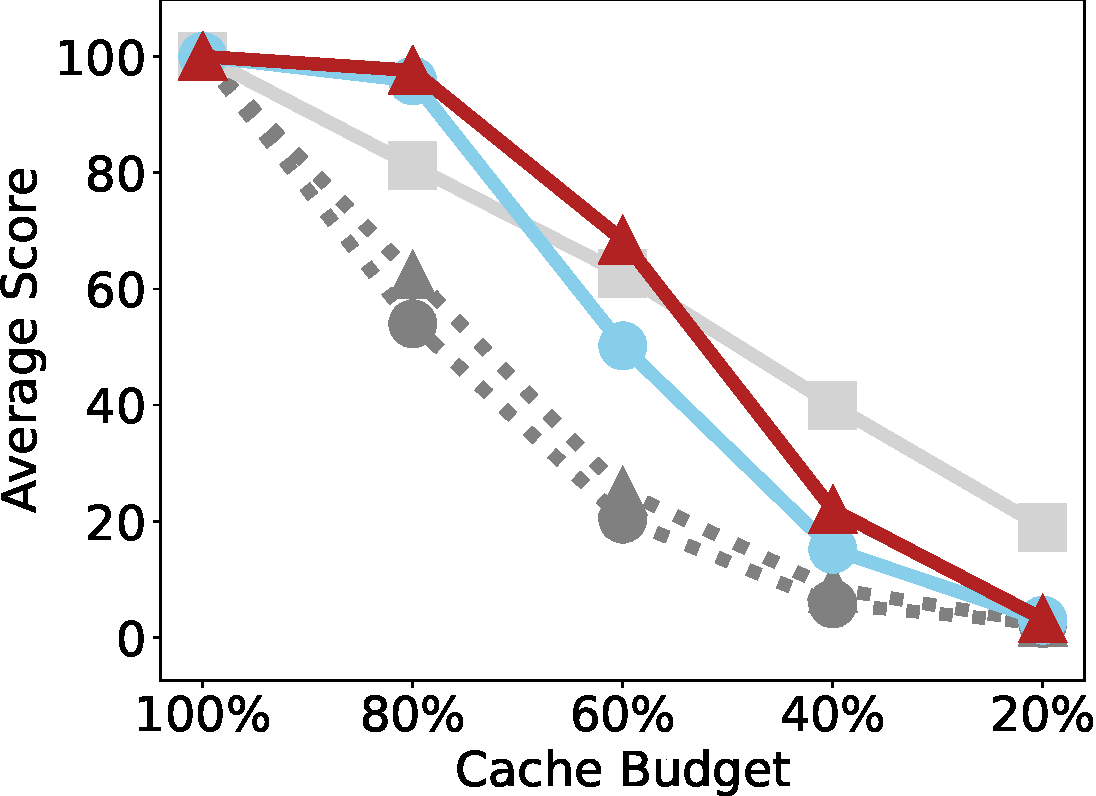
\includegraphics[width=\linewidth]{./Figures/ruler_per_dataset_group_by_wq/niah_single_3_Llama3.1_ruler_score.pdf}
	\vspace{-0.4cm}
	\caption{S-NIAH-3}
	\label{subfig:sniah3}
	\end{subfigure}
	\begin{subfigure}[b]{0.16\linewidth}
	\centering
	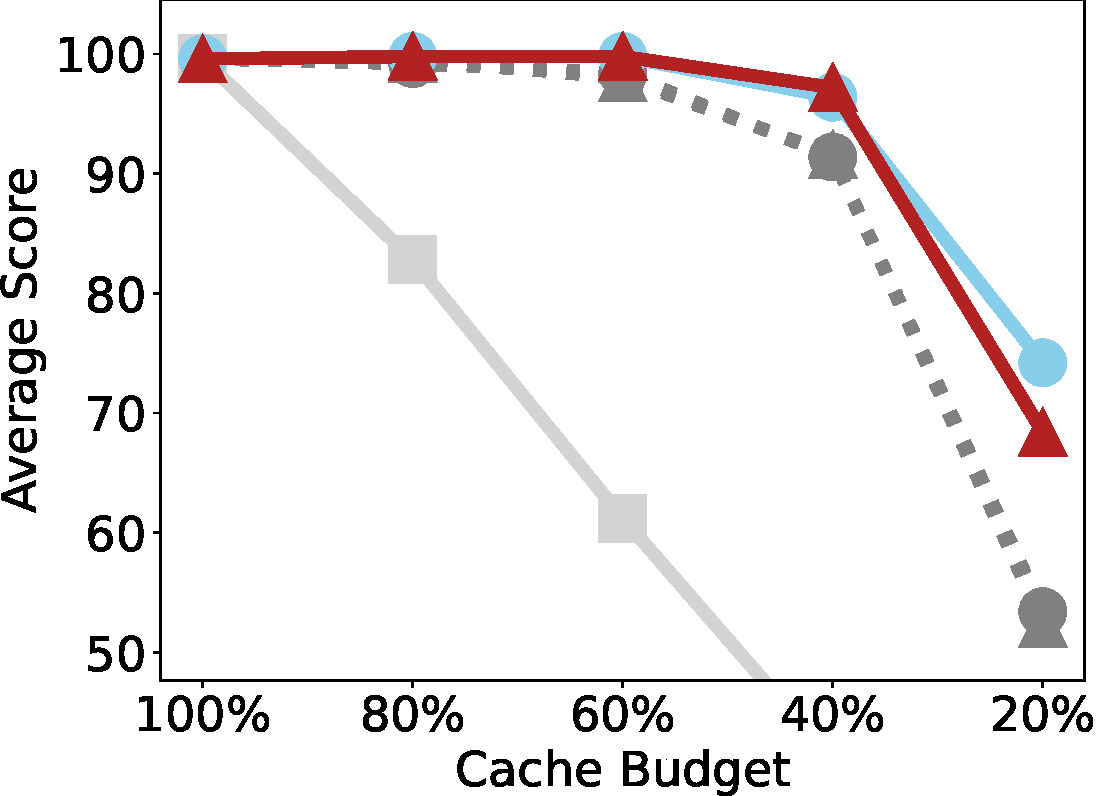
\includegraphics[width=\linewidth]{./Figures/ruler_per_dataset_group_by_wq/niah_multikey_1_Llama3.1_ruler_score.pdf}
	\vspace{-0.4cm}
	\caption{MK-NIAH-1}
	\end{subfigure}
	\begin{subfigure}[b]{0.16\linewidth}
	\centering
	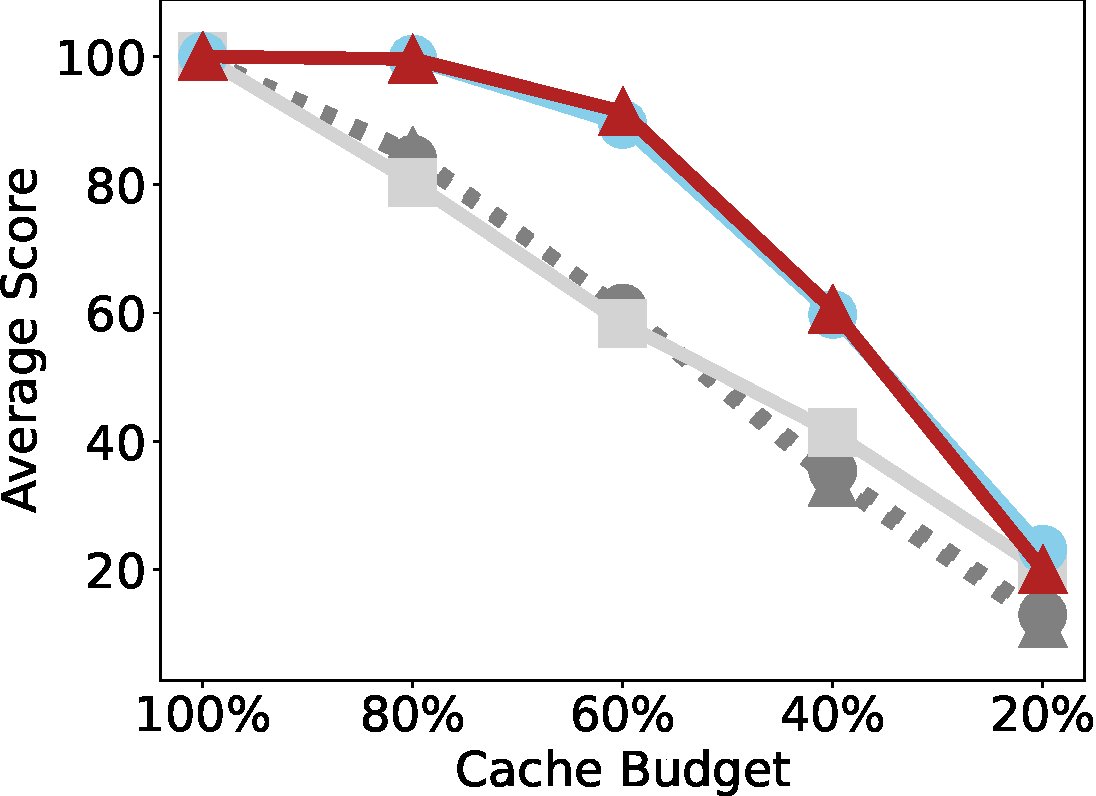
\includegraphics[width=\linewidth]{./Figures/ruler_per_dataset_group_by_wq/niah_multikey_2_Llama3.1_ruler_score.pdf}
	\vspace{-0.4cm}
	\caption{MK-NIAH-2}
	\label{subfig:mkniah2}
	\end{subfigure}
	\begin{subfigure}[b]{0.16\linewidth}
	\centering
	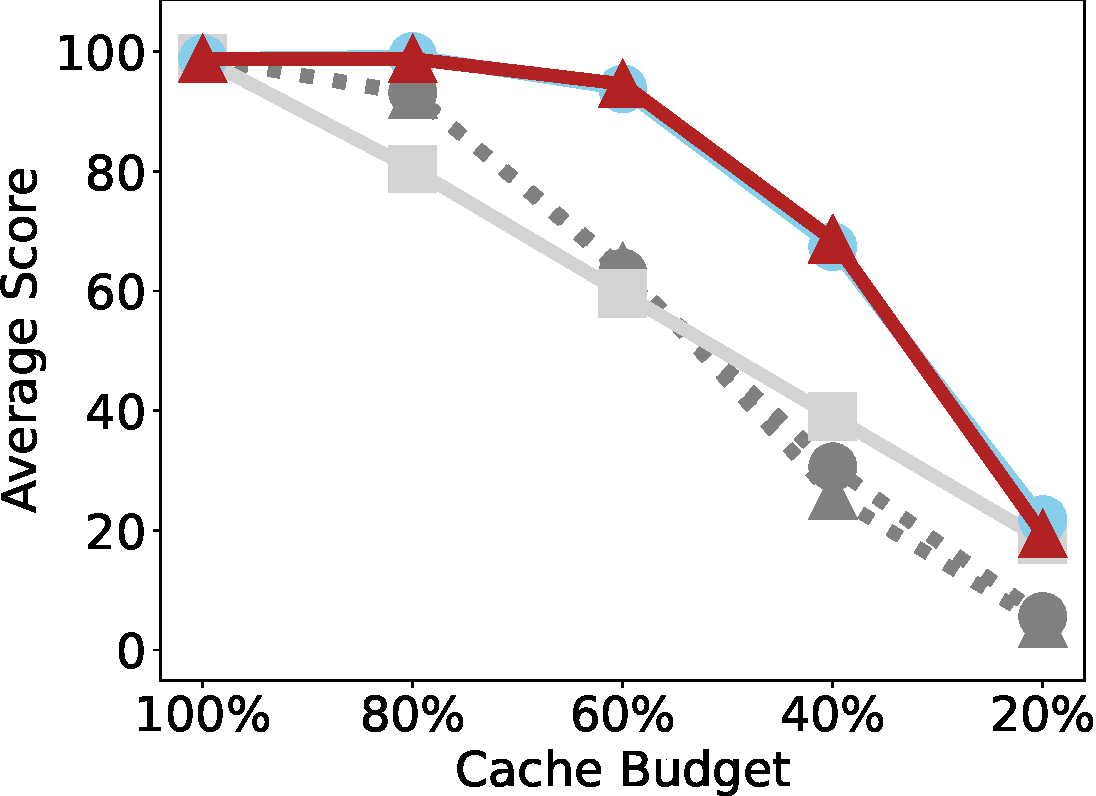
\includegraphics[width=\linewidth]{./Figures/ruler_per_dataset_group_by_wq/niah_multikey_3_Llama3.1_ruler_score.pdf}
	\vspace{-0.4cm}
	\caption{MK-NIAH-3}
	\end{subfigure}
	\begin{subfigure}[b]{0.16\linewidth}
	\centering
	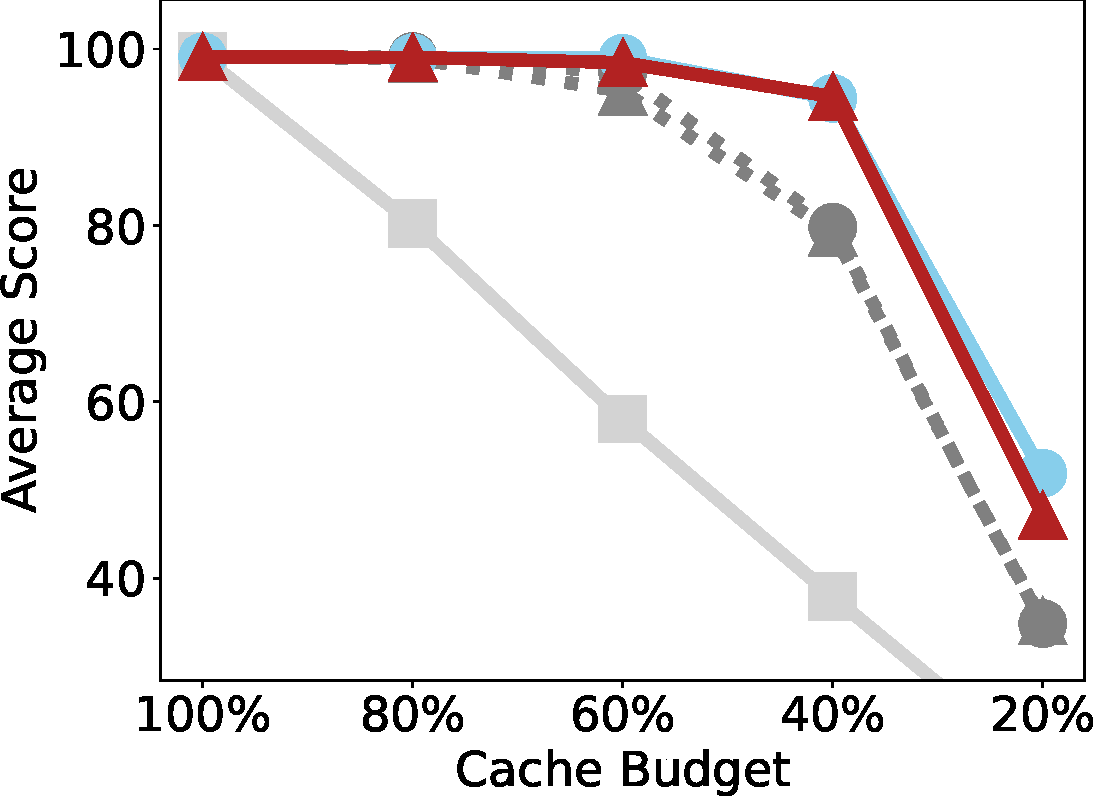
\includegraphics[width=\linewidth]{./Figures/ruler_per_dataset_group_by_wq/niah_multivalue_Llama3.1_ruler_score.pdf}
	\vspace{-0.4cm}
	\caption{MV-NIAH}
	\end{subfigure}
	\begin{subfigure}[b]{0.16\linewidth}
	\centering
	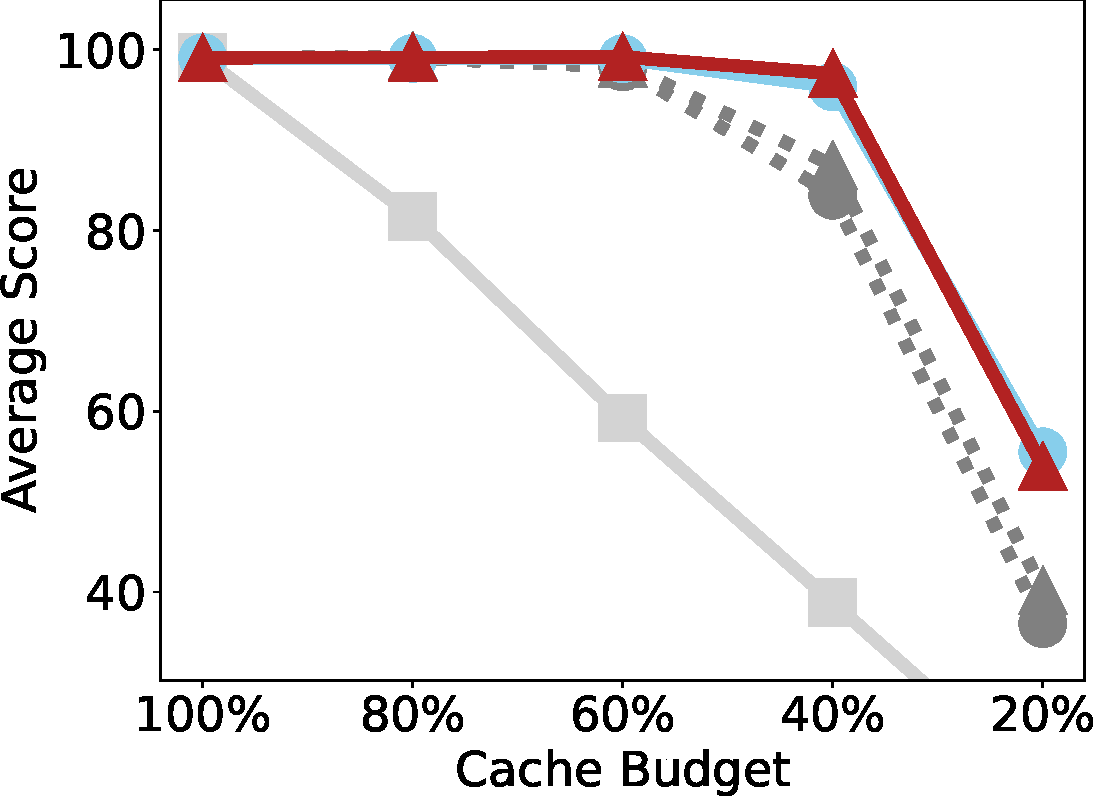
\includegraphics[width=\linewidth]{./Figures/ruler_per_dataset_group_by_wq/niah_multiquery_Llama3.1_ruler_score.pdf}
	\vspace{-0.4cm}
	\caption{MQ-NIAH}
	\end{subfigure}
	\begin{subfigure}[b]{0.16\linewidth}
	\centering
	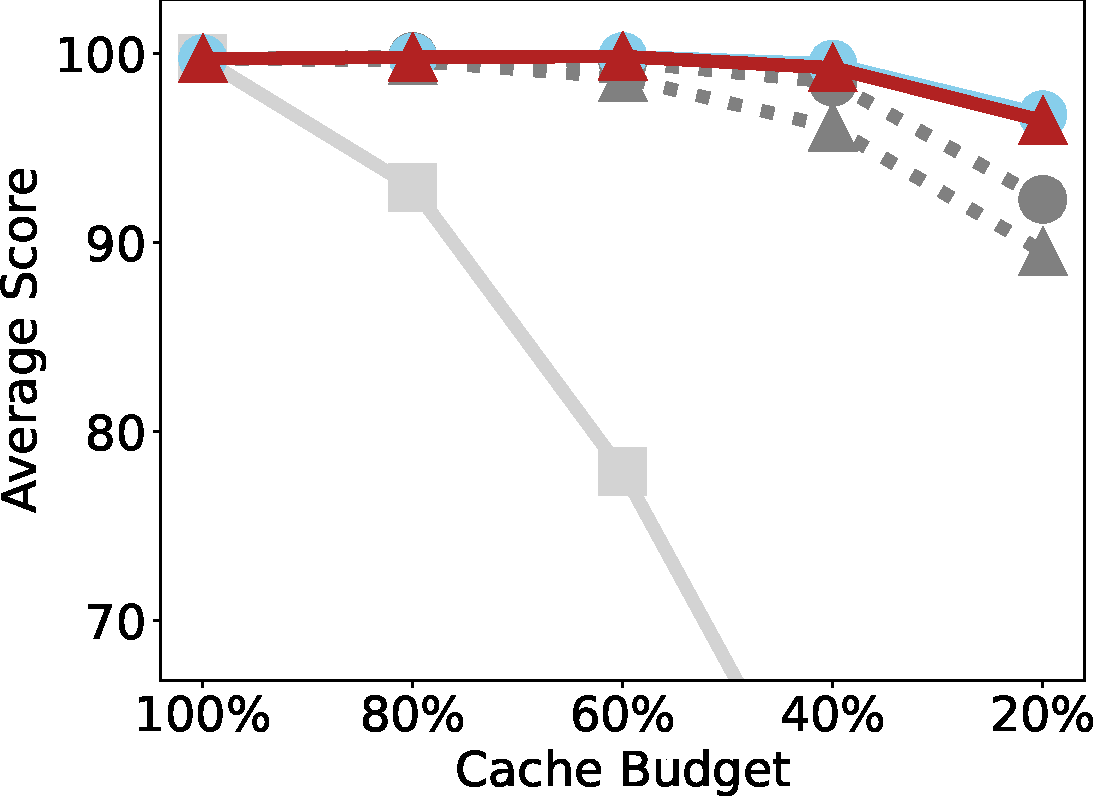
\includegraphics[width=\linewidth]{./Figures/ruler_per_dataset_group_by_wq/vt_Llama3.1_ruler_score.pdf}
	\vspace{-0.4cm}
	\caption{VT}
	\end{subfigure}
	\begin{subfigure}[b]{0.16\linewidth}
	\centering
	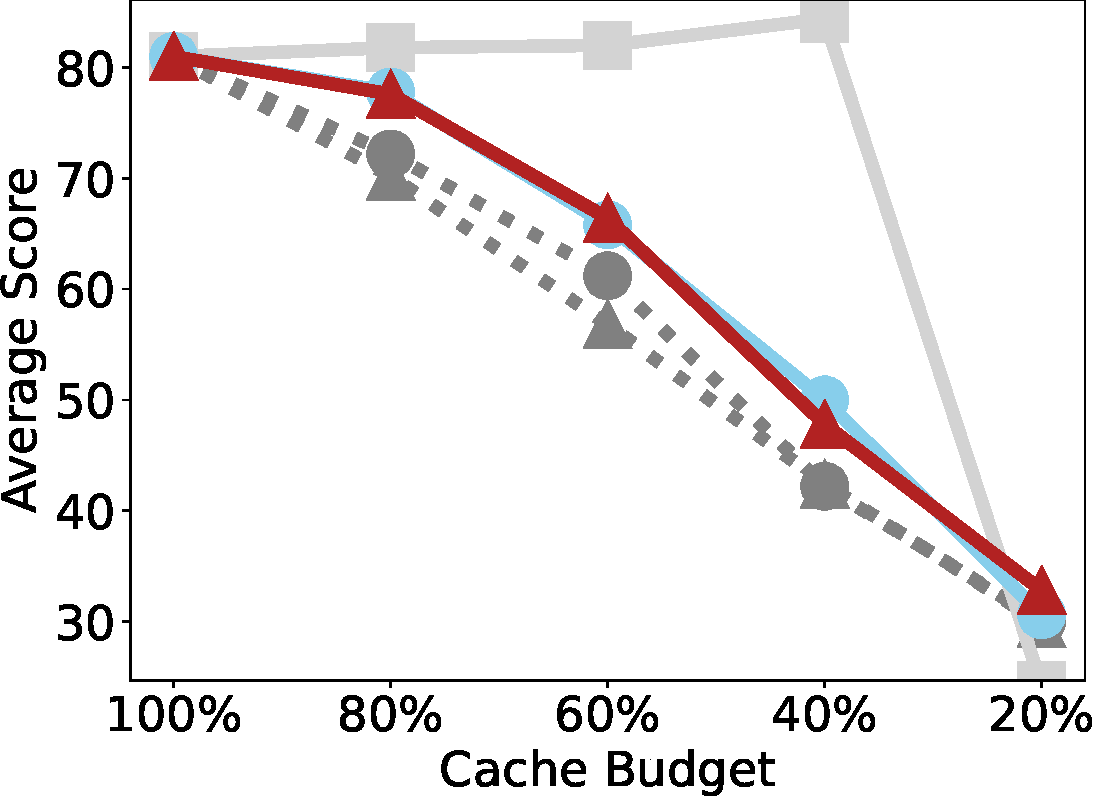
\includegraphics[width=\linewidth]{./Figures/ruler_per_dataset_group_by_wq/qa_1_Llama3.1_ruler_score.pdf}
	\vspace{-0.2cm}
	\caption{S-QA}
	\end{subfigure}
	\vspace{-0.1cm}
	\caption{Subtask Analysis on Ruler (Question-agnostic, Llama-3.1-8B-Instruct).}
	\label{fig:agnostic_llama_ruler_subtask}
	\vspace{-0.2cm}
\end{figure*}

\subsection{Ruler Benchmark}
We evaluate quality scores for each method using budgets set to 20\%, 40\%, 60\%, and 80\% of the original cache size. Beyond the commonly studied \textbf{question-aware} compression scenario—where questions are known in advance—we also consider the more challenging \textbf{question-agnostic} setting~\cite{kvpress}, in which questions are revealed only after compression.
This  mimics more challenging scenarios, such as prompt caching~\cite{gim2024prompt,zheng2024sglang}, where numerous question-independent prefix prompts need compression, or multi-turn dialogue~\cite{yi2024survey}, where compression occurs without future questions.



\textbf{Overall Results.}
Figure~\ref{fig:ruler_ave} presents the average scores across 13 datasets in the Ruler Benchmark.
Overall, existing Top-k eviction methods exhibit significant performance drops in the question-agnostic scenario.
In contrast, our Ada-SnapKV and Ada-Pyramid consistently outperform the original SnapKV and Pyramid across both question-aware and question-agnostic scenarios on the two LLMs.
Using the Llama-3.1-8B-Instruct model as an example: in the simpler question-aware scenario (Figure~\ref{fig:aware_llama}), both Ada-SnapKV and Ada-Pyramid significantly reduce quality loss under small compression budgets, such as 40\% and 20\% cache sizes, compared to the original SnapKV and Pyramid. In the more challenging question-agnostic scenario (Figure~\ref{fig:agnostic_llama}), Ada-SnapKV and Ada-Pyramid substantially reduce quality loss across all cache budget settings.
For instance, leveraging the adaptive allocation strategy, Ada-SnapKV improves SnapKV's scores at 80\% and 20\% cache sizes from 87.59 and 44.02 to 92.67 and 53.29, respectively.





\textbf{Subtask Analysis.}
Figure \ref{fig:agnostic_llama_ruler_subtask} presents the results for 12 datasets using Llama-3.1-8B-Instruct in the challenging question-agnostic scenario, highlighting the improvements brought by the adaptive budget allocation strategy. More results are provided in Appendix \ref{apdx:detail_ruler}, where our method also shows significant improvements.
Overall, our adaptive budget allocation strategy significantly enhances the performance of existing methods.
For example, at 80\% cache budget, the original SnapKV demonstrates noticeable degradation on many tasks, whereas Ada-SnapKV maintains near-lossless performance across most tasks.
Particularly in difficult Needle-in-a-Haystack tasks like S-NIAH-3 and MK-NIAN-2 with 80\% cache budget, Ada-SnapKV increases SnapKV's scores from 62.4 and 85.2 to 97.6 and 99.6, as shown in Figures~\ref{subfig:sniah3} and \ref{subfig:mkniah2}.
 These results emphasize the effectiveness of incorporating adaptive budget allocation for enhancement, especially in difficult tasks.




 \begin{figure*}[tp]
\vspace{-0.2cm}
	\begin{minipage}{\linewidth}
		\centering
		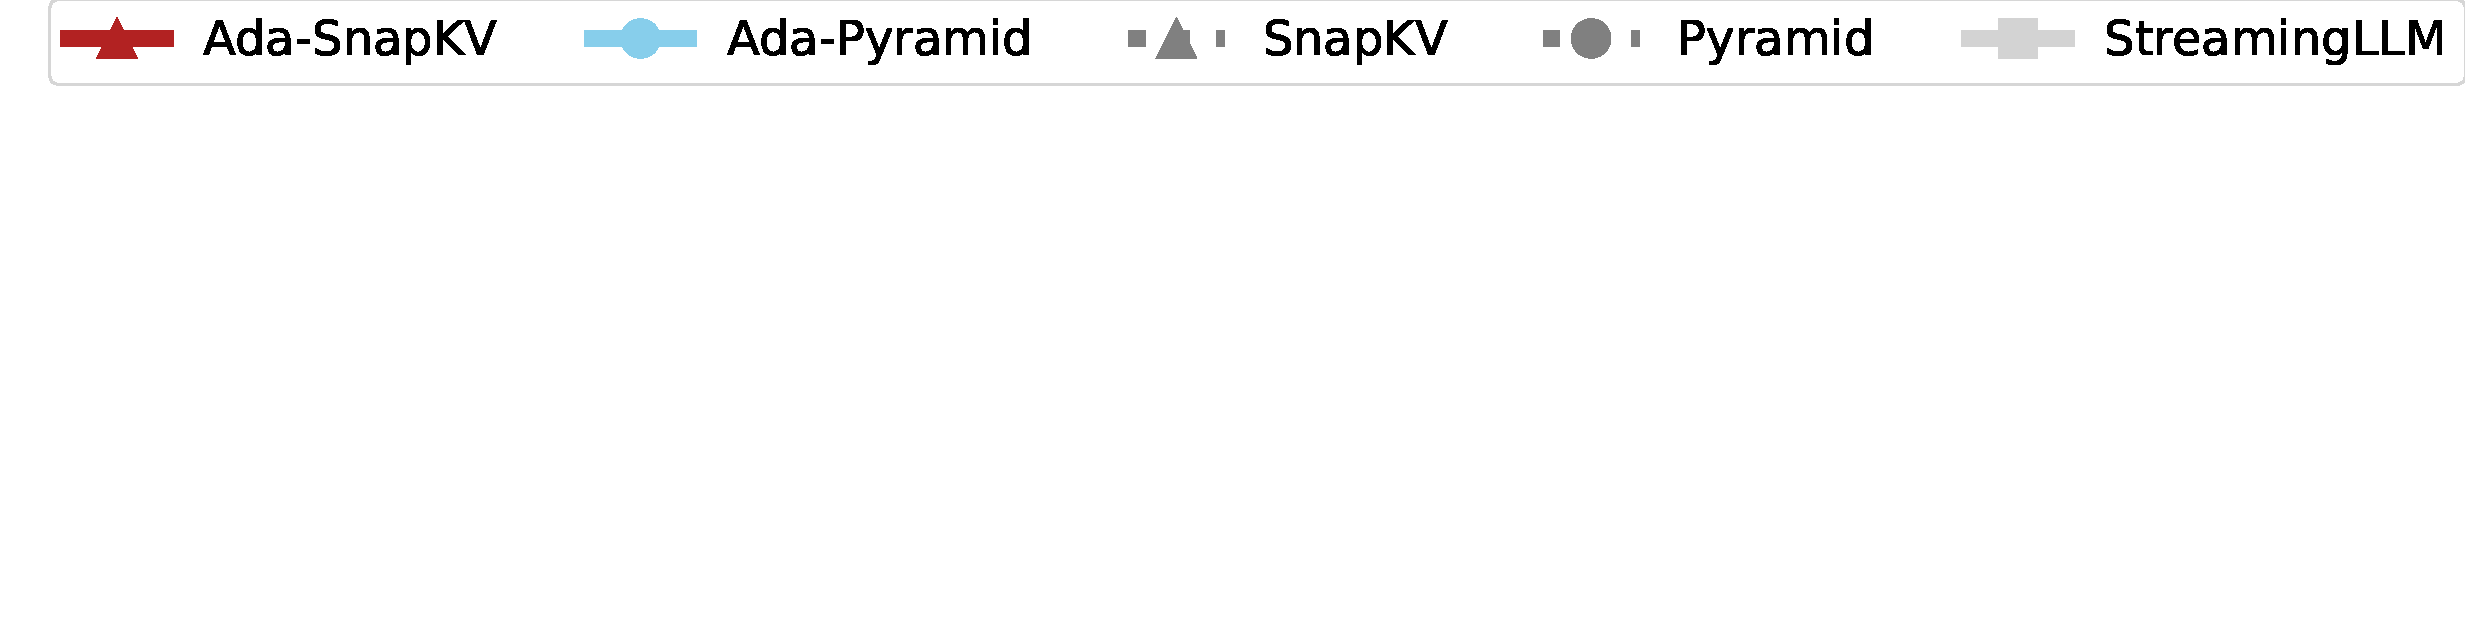
\includegraphics[width=0.85\linewidth]{./Figures/ruler_per_dataset_group_by_wq/legend.pdf}
	\end{minipage}
	\centering
	\begin{subfigure}[b]{0.24\linewidth}
		\centering
		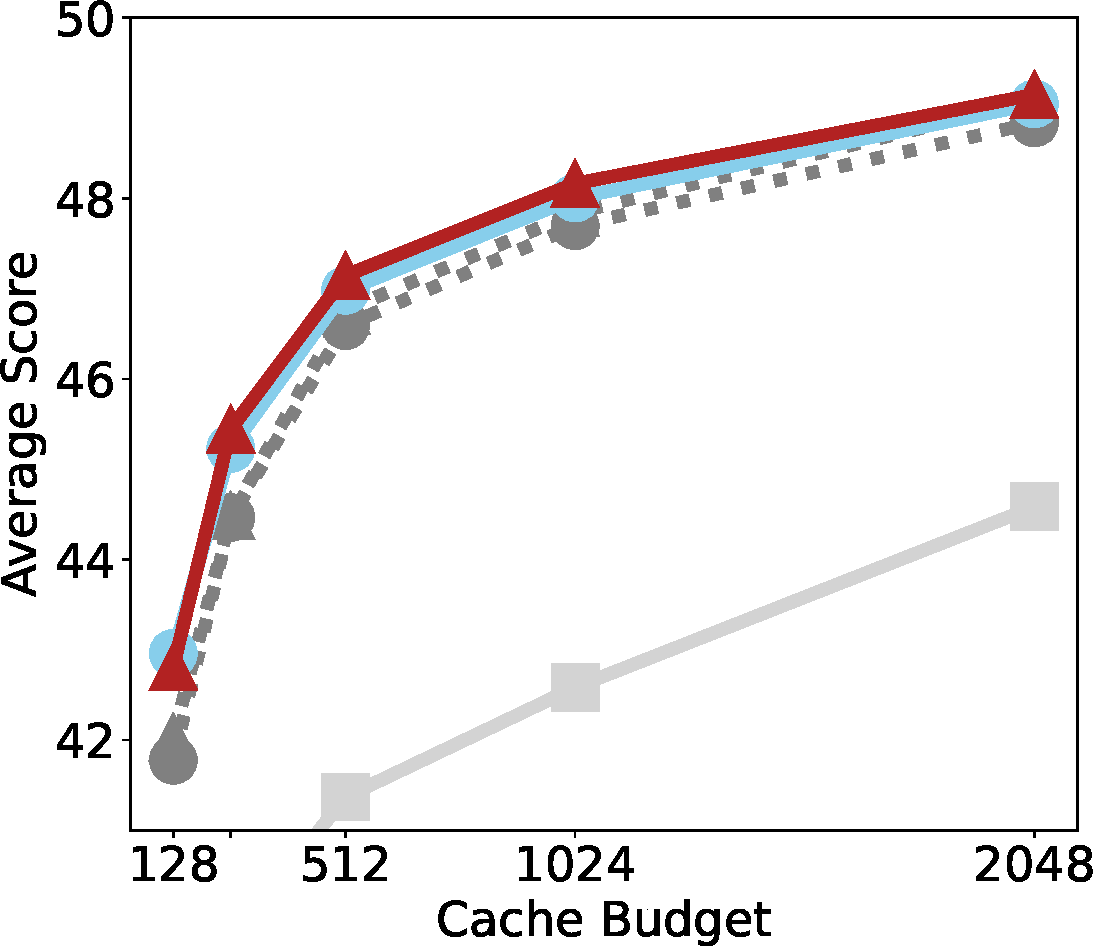
\includegraphics[width=\linewidth]{./Figures/Llama3.1_longbench_score.pdf}
		\vspace{-0.3cm}	
		\caption{\centering  Question-aware \newline Llama-3.1-8B-Instruct}
		\label{fig:quest_aware_llama_ave_quality_loss}
	\end{subfigure}
	\begin{subfigure}[b]{0.24\linewidth}
		\centering
		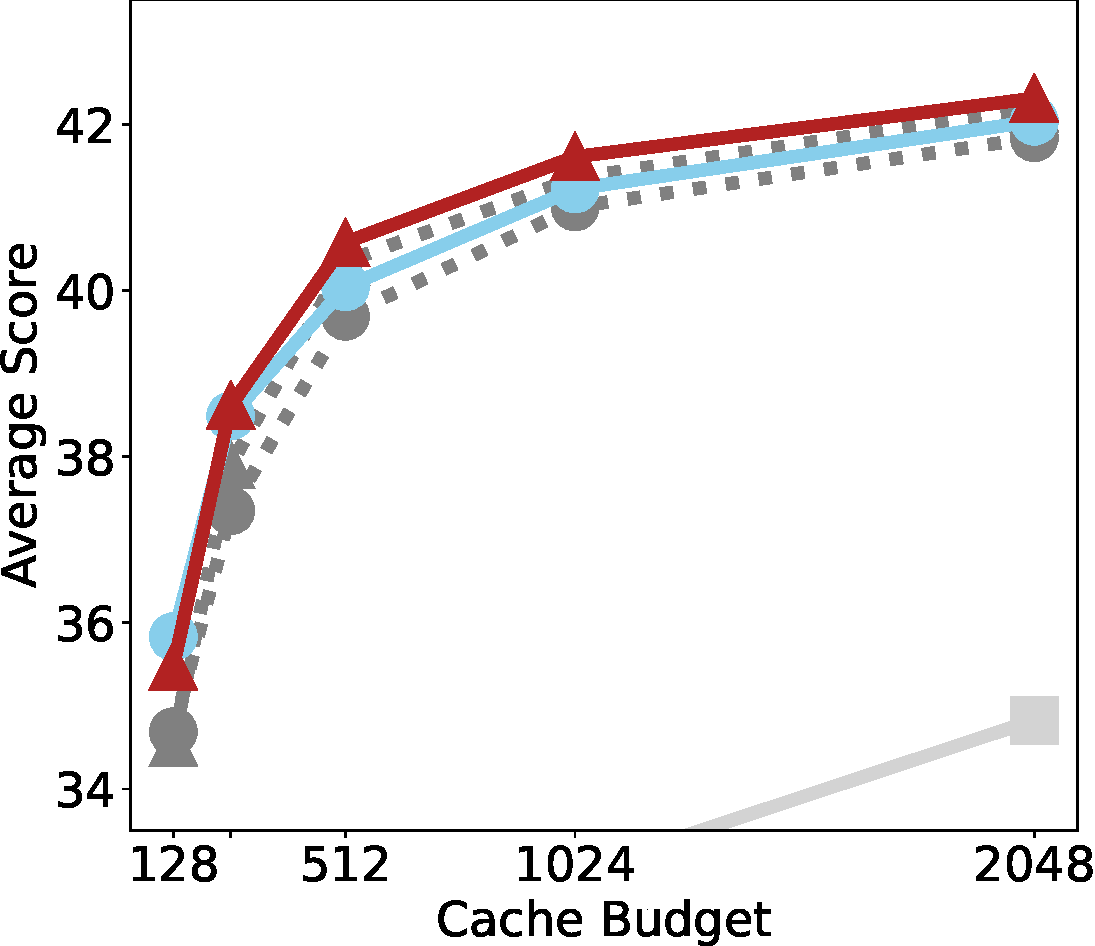
\includegraphics[width=\linewidth]{./Figures/Mistral_longbench_score.pdf}
		\vspace{-0.3cm}
		\caption{\centering Question-aware \newline Mistral-7B-Instruct-v0.2}
		\label{fig:quest_aware_mistral_ave_quality_loss}
	\end{subfigure}
	\begin{subfigure}[b]{0.24\linewidth}
		\centering
		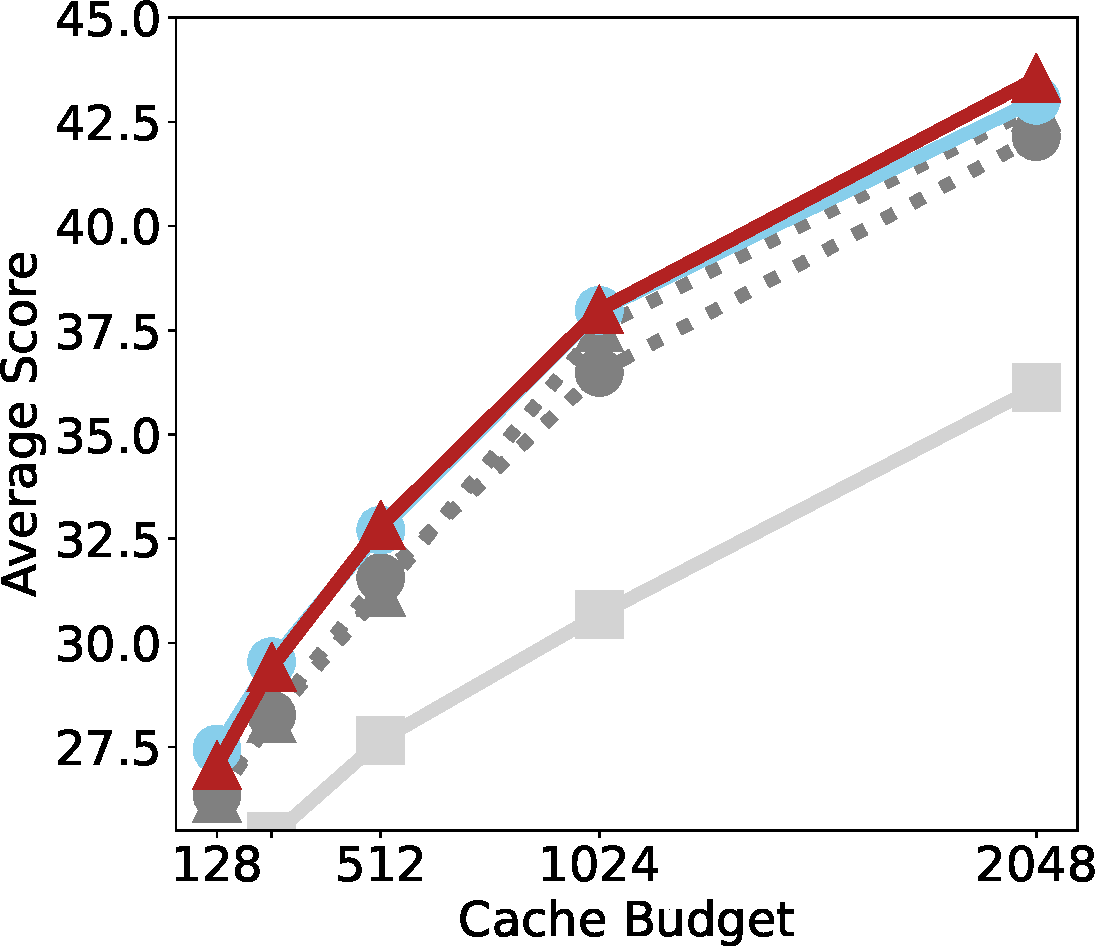
\includegraphics[width=\linewidth]{./Figures/longbench/Llama3.1_longbench_score_question_agnostic.pdf}
		\vspace{-0.3cm}
		\caption{\centering Question-agnostic \newline Llama-3.1-8B-Instruct}
			\label{fig:quest_agnostic_llama_ave_quality_loss}
	\end{subfigure}
	\begin{subfigure}[b]{0.24\linewidth}
		\centering
		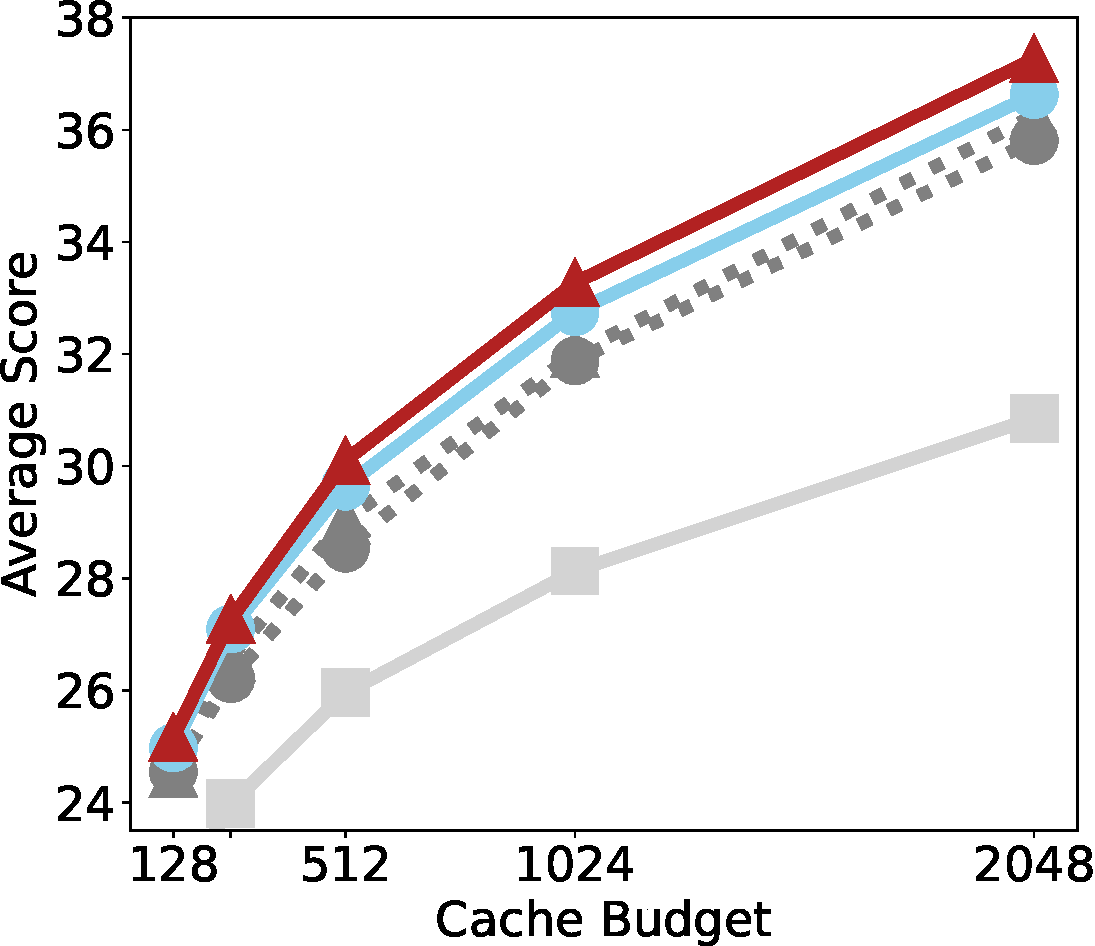
\includegraphics[width=\linewidth]{./Figures/longbench/Mistral_longbench_score_question_agnostic.pdf}
		\vspace{-0.3cm}
		\caption{\centering Question-agnostic \newline Mistral-7B-Instruct-v0.2}
		\label{fig:quest_agnostic_mistral_ave_quality_loss}
	\end{subfigure}
	
	\vspace{-0.1cm}
	\caption{Average Score on LongBench among 16 Datasets under Fixed Budgets.}
	\label{fig:ave_quality_loss}
	\vspace{-0.3cm}
\end{figure*}





\begin{table}[t!]  
	\centering  
	\small
	\vspace{-0.2cm}
	\caption{Task Analysis for Llama-3.1-8B (Question-agnostic).}  
	\label{tab:comparison_ratio_budget}  
	\resizebox{\textwidth}{!}{ 
	\begin{tabular}{@{}l c ccc ccc@{}}  
		\toprule  
		\multirow{2}{*}{Task Domains} & \multirow{2}{*}{\makecell{Full\\Cache}} & \multicolumn{2}{c}{$b=10\%$} & \multicolumn{2}{c}{$b=20\%$} & \multicolumn{2}{c}{$b=40\%$} \\
		\cmidrule(lr){3-4}\cmidrule(lr){5-6}\cmidrule(lr){7-8}  
		& & SnapKV & Ada-SnapKV & SnapKV & Ada-SnapKV & SnapKV & Ada-SnapKV \\
		\midrule  
		Single-Doc. QA & 43.10 & 23.38 & \textbf{23.97} & 28.78 & \textbf{31.39} & 35.27 & \textbf{36.63} \\
		Multi-Doc. QA  & 46.49 & 26.61 & \textbf{29.06} & 33.51 & \textbf{34.90} & 40.50 & \textbf{41.36} \\
		Summarization  & 28.97 & 21.98 & \textbf{22.43} & 23.82 & \textbf{24.29} & 26.11 & \textbf{26.66} \\
		Few-shot       & 69.45 & 57.89 & \textbf{60.40} & 61.95 & \textbf{63.70} & 65.10 & \textbf{66.43} \\
		Synthetic      & 53.73 & \textbf{36.50} & 34.88 & 48.19 & \textbf{50.39} & \textbf{53.17} & 53.00 \\
		Code           & 57.86 & 59.72 & \textbf{60.91} & 60.05 & \textbf{61.14} & \textbf{60.49} & 60.30 \\
		\hline  
		Ave.           & 49.20 & 36.38 & \textbf{37.45} & 41.29 & \textbf{42.87} & 45.52 & \textbf{46.24} \\
		\bottomrule  
	\end{tabular}  
}
\vspace{-0.3cm}
\end{table}

\subsection{LongBench Benchmark}
To align with previous evaluations~\cite{SnapKV,PyramidKV}, we first set the average budget for each head to fixed values of $\{128 , 256 , 512 , 1024, 2048\}$.
We further extend from standard question-aware compression to question-agnostic scenarios by separating the questions in Longbench, thereby better reflecting real-world performance, as suggested by~\cite{kvpress}. 
For more details, please refer to Appendix \ref{apdx:longbench_info}.



\textbf{Question-aware Compression:} Figures~\ref{fig:quest_aware_llama_ave_quality_loss} and \ref{fig:quest_aware_mistral_ave_quality_loss} present the average scores across 16 datasets under fixed budget constraints with the question-aware compression.~\footnote{Detailed scores can be found in Appendix \ref{apdx:detail_LongBench}}. SnapKV and Pyramid, both utilizing Top-$k$ selection within an observation window, achieve closely matched performance and outperform the previous sliding window eviction method, StreamingLLM. Moreover, our Ada-SnapKV and Ada-Pyramid methods consistently improve generation quality across different budgets, alternately outperforming their respective base methods and, under a fixed budget of 2048, approaching lossless performance. These consistent gains highlight the effectiveness of adaptive budget allocation.


\textbf{From Question-aware to Question-agnostic Compression:} Figures~\ref{fig:quest_agnostic_llama_ave_quality_loss} and \ref{fig:quest_agnostic_llama_ave_quality_loss} further present the average scores with the question-agnostic compression. Our enhanced Ada-SnapKV and Ada-Pyramid methods continue to outperform the original SnapKV and Pyramid methods. However, a comparison between question-aware and question-agnostic settings reveals a notable performance drop across all methods. For example, with Llama and a 2048 budget, the average score of SnapKV decreases from 49.09 to 42.86 while transfer from question-aware to question-agnostic settings. This indicates that commonly used question-aware settings do not adequately capture the limitations of cache eviction methods in a more realistic compression scenario. We therefore suggest that future evaluations of cache eviction techniques should place greater emphasis on question-agnostic compression to improve robustness in practical applications.



\textbf{More Evaluation in Question-agnostic Compression:}  
To more accurately assess question-agnostic compression, we apply ratio-based cache budget compression, which better reflects real-world performance on Longbench’s highly imbalanced sample lengths. \footnote{As shown in Table~\ref{tab:information_dataset} (Appendix~\ref{apdx:longbench_info}), Longbench sample lengths are highly imbalanced—for example, the Code task Lcc averages 1,235 tokens, while the QA task NarrativeQA averages 18,409. Thus, applying a fixed budget, like 2048, across all datasets may introduce bias when evaluating cache eviction across tasks.} Table~\ref{tab:comparison_ratio_budget} provides a detailed breakdown of performance across task domains for Llama-3.1-8B. Overall, Code tasks are largely insensitive to cache compression, and in some cases, even see improved performance after compression. In contrast, other tasks experience significant degradation, particularly in Summarization and QA. Notably, our Ada-SnapKV effectively mitigates these losses and improves overall performance. Across 18 domain cases and three cache budgets, Ada-SnapKV delivers quality improvements in 15 domains, demonstrating its robust benefits. Table~\ref{tab:comparison_ratio_budget_70b} further reports results on the larger Llama-3.1-70B model, showing similarly strong gains from our approach. Except for the Code domain, which remains insensitive to compression, significant improvements are observed in all other tasks.




\begin{figure}[t]  
	\begin{minipage}[t]{0.685\textwidth}  
		
				\vspace{0pt}  
		\centering  
		\small  
		\setlength{\tabcolsep}{3pt}  
		\captionof{table}{Task Analysis for Llama-3.1-70B (Question-agnostic).}  
		\vspace{-0.2cm}
		\label{tab:comparison_ratio_budget_70b}  
	 	\resizebox{\textwidth}{!}{  

			\begin{tabular}{@{}l c c c c c@{}}  
				\toprule  
				\multirow{2}{*}{Domain} & \multirow{2}{*}{\makecell{Full Cache}} & \multicolumn{2}{c}{\small \makecell{$b =$ 20\%}} & \multicolumn{2}{c}{\small \makecell{$b =$ 40\%}} \\
				\cmidrule(lr){3-4}\cmidrule(lr){5-6}  
				& & SnapKV  & Ada-SnapKV & SnapKV  & Ada-SnapKV \\
				    \midrule  
				Single-Doc. QA & 47.15 & 32.54 & \textbf{36.05} & 39.35 & \textbf{42.21} \\
				Multi-Doc. QA & 60.07 & 46.98 & \textbf{48.45} & 54.07 & \textbf{55.03} \\
				Summarization & 28.69 & 24.40 & \textbf{24.81} & 26.21 & \textbf{26.57} \\
				Few-shot & 72.07 & 66.71 & \textbf{67.80} & 69.29 & \textbf{70.29} \\
				Synthetic & 58.25 & 51.25 & \textbf{51.50} & 56.00 & \textbf{56.75} \\
				Code & 47.82 & \textbf{52.44} & 51.51 & \textbf{51.90} & 49.23 \\
				\midrule  
				Ave. & 52.25 & 44.95 & \textbf{46.08} & 48.91 & \textbf{49.64} \\
				\bottomrule  
			\end{tabular}  }
	\end{minipage}%  
	\begin{minipage}[t]{0.28\textwidth}  
		\vspace{0pt}  
		\centering  
		\begin{subfigure}{0.98\linewidth}  
			\centering  
			\includegraphics[width=0.99\linewidth]{./Figures/MemConsumption.pdf}  
			\vspace{-0.6cm}  
			\captionsetup{labelformat=empty} 
			\caption{\small Memory}  
		\end{subfigure}  
		\begin{subfigure}{0.98\linewidth}  
			\centering  
			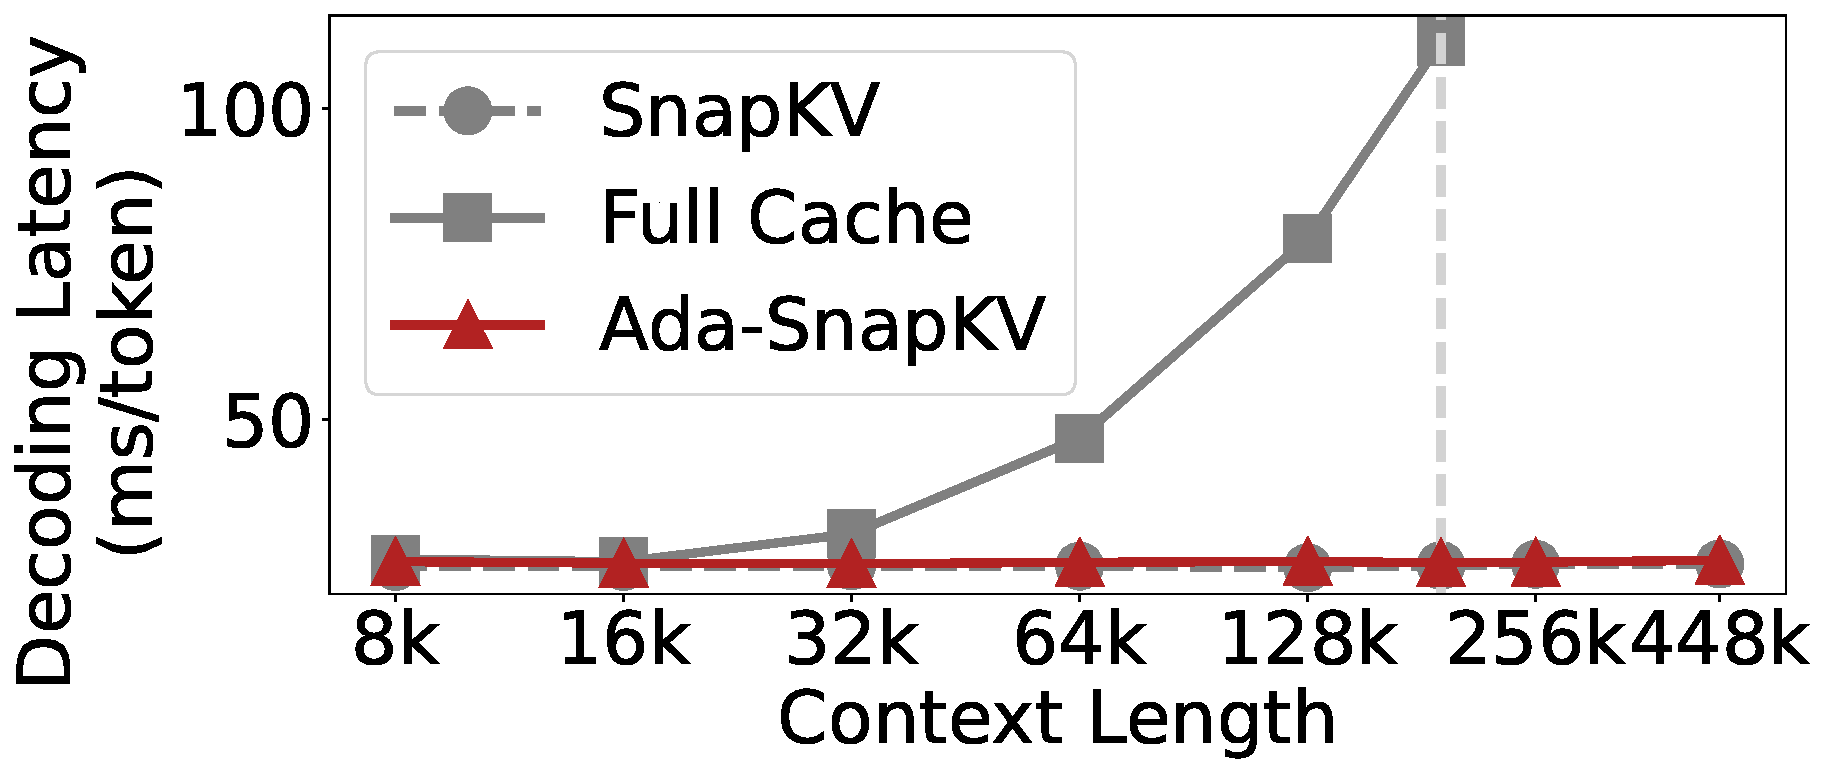
\includegraphics[width=0.99\linewidth]{./Figures/DecodingSpeed.pdf}  
			\vspace{-0.6cm}  
			\captionsetup{labelformat=empty} 
			\caption{\small Runtime}  
		\end{subfigure}  
		\vspace{-0.2cm}  
		\caption{\centering Efficiency  {\small (All with FlashAttention-2)}}  
		\label{fig:efficiency}  
	\end{minipage}  
	\vspace{-0.5cm}
\end{figure}





\subsection{Computation Efficiency Under Adaptive Allocation}
\label{sc:exp_efficiency}
Cache eviction methods aim to enhance the computational (memory and runtime) efficiency by selectively evicting KV cache elements.
We demonstrate that, supported by our flattened cache layout and custom CUDA kernels, the computational efficiency of cache eviction under adaptive allocation, based on the variable-length FlashAttention technique, matches that of traditional uniform eviction methods within the same cache budget constraints.
As shown in Figure \ref{fig:efficiency}, with a fixed budget of 1024, Ada-SnapKV achieves peak memory usage and decoding latency comparable to the original SnapKV, and both  significantly outperform the full cache case.
These results demonstrate that Ada-KV strategy effectively enhance post-eviction generation quality while maintaining strong computational efficiency.



\section{Broad Benefits of the Adaptive Budget Allocation Strategy}
\label{sc:broad}
Due to its plug-and-play design, Ada-KV is broadly applicable beyond the two cases presented in this paper. As of publication, many follow-up works have adopted Ada-KV strategy, yielding a wide range of enhanced applications~\cite{kim2025kvzip, devoto2025expected,galim2025draft}, especially CriticalKV~\cite{feng2025identify} and DefensiveKV~\cite{feng2025tamingfragilitykvcache}.
Beyond direct integration, concurrent methods have explored budget allocation through training-based profiling. For instance, DuoAttention~\cite{xiao2024duoattention} categorizes heads into “full attention” and “streaming” types, while HeadKV~\cite{fu2024not} enables finer-grained allocation building on our open-source implementation. We present the results of these follow-up studies in Table~\ref{tab:follow_up} to demonstrate the broad benefits of adaptive budget allocation strategy. When combined with CriticalKV and DefensiveKV, Ada-KV consistently improves performance, which in turn scales with the strength of the base method. Notably, even the plug-and-play CriticalKV and DefensiveKV methods, when enhanced with the Ada-KV strategy, surpass the performance of training-based approaches like DuoAttention and HeadKV. These findings demonstrate that Ada-KV retains substantial value and offers significant enhancement potential, even alongside more recent and advanced methods.


 \begin{table}[t!]  
	\centering
	\small  
	\caption{Performance gains from applying the Ada-KV strategy to follow-up methods. All results are from the Llama-3.1-8B model on the Longbench benchmark under question-agnostic settings.}  
	\label{tab:follow_up}  
	\begin{tabular}{@{}lcccccc@{}}  
		\toprule  
		{Cache} & {\begin{tabular}[c]{@{}c@{}} DuoAttn\\ {\scriptsize \textit{Training-based}}\end{tabular}} & {\begin{tabular}[c]{@{}c@{}}HeadKV\\ {\scriptsize \textit{Training-based}}\end{tabular}} & {\begin{tabular}[c]{@{}c@{}}CriticalKV\\ {w/o. Ada-KV}\end{tabular}} & {\begin{tabular}[c]{@{}c@{}}CriticalKV\\ {w/. Ada-KV}\end{tabular}} & {\begin{tabular}[c]{@{}c@{}}DefensiveKV\\ {w/o. Ada-KV}\end{tabular}}  & {\begin{tabular}[c]{@{}c@{}}DefensiveKV\\ {w/. Ada-KV}\end{tabular}} \\
		\midrule  
		20\% & 39.52 & 42.64 & 42.99 & 43.77 & 43.78 & \textbf{46.68} \\
		40\% & 48.17 & 47.23 & 47.29 & 48.00 & 47.76 & \textbf{49.21} \\
		\bottomrule  
	\end{tabular}  
	\vspace{-0.2cm}
\end{table} 